\documentclass[12pt]{article}
\usepackage[T1]{fontenc}
\usepackage[utf8]{inputenc}
\usepackage{lmodern}
\usepackage[margin=1.15in]{geometry}
\usepackage{amsmath,amssymb,booktabs,threeparttable,microtype,setspace,enumitem,natbib,graphicx}
\usepackage{xcolor,hyperref}
\hypersetup{colorlinks=true,linkcolor=blue!50!black,citecolor=blue!50!black,urlcolor=blue!50!black,pdftitle={From Competing Pension Regimes to Pillars or Full Funding},pdfauthor={Oliver Pardo}}
\onehalfspacing
\newcommand{\1}{\mathbf{1}}
\newcommand{\dd}{\,\mathrm{d}}

\title{\textbf{From Competing Pension Regimes to Pillars or Full Funding:}\\
\large Informality, Fiscal Transition, and Welfare in Colombia}
\author{Oliver Pardo\thanks{Departamento de Administraci{\'o}n, Pontificia Universidad Javeriana,
Bogot{\'a}, Colombia. Email: \href{mailto:pardoo@javeriana.edu.co}{pardoo@javeriana.edu.co}.}}
\date{August 2026}

\begin{document}
\maketitle

\begin{abstract}\small\sloppy
\noindent
This paper studies Colombia's counterfactual transition from the competing pension regimes
created by Law 100 of 1993 to two alternatives: the pillar architecture of Law 2381 of 2024
and a fully funded formal system. I embed endogenous informality, PAYG eligibility, portable
funded balances, voluntary saving, public debt, and general-equilibrium prices in a two-period
overlapping-generations economy. The fiscal block maps Colombia's statutory 55 percent
net-debt anchor and 0.2 percent structural primary surplus into a 40-year model period. A
smooth consumption wedge and a separate primary-balance adjustment stabilize debt without
forcing the consumption tax to absorb each PAYG shock contemporaneously. In the Law 100
steady state, informality is 53.2 percent and funded accounts hold 77.0 percent of household
assets. Under pillars, informality rises to 77.9 percent, capital falls 14.1 percent, and the
stationary consumption tax is 55.4 percent. Funded saving falls by 70.3 percent, but voluntary
saving rises by 173.8 percent. The high tax is therefore not explained by the disappearance of
all nonpension saving or by a larger net PAYG deficit; it mainly reflects the endogenous
contraction of the consumption-tax base and other fiscal revenue. The transition is damped
and converges to the debt anchor. In the fully funded counterfactual, informality falls to
10.2 percent, capital more than doubles, and stationary welfare rises 22.9 percent in
consumption-equivalent terms. Its negative 3.0 percent residual fiscal wedge is a model-implied
dividend, not a proposed negative VAT. These comparisons identify mechanisms rather than
provide forecasts: one model period spans a generation, domestic public debt does not crowd
out household capital in the central specification, and Law 2381 has not been implemented.

\medskip\noindent\textbf{Keywords:} pension reform; informality; pillar system; PAYG; funded accounts;
public debt; transitional dynamics; distributional welfare. \quad \textbf{JEL:} E21; H55; J26; J46.
\end{abstract}\fussy

\section{Introduction}

Workers in economies with large informal sectors choose both whether to enter formal employment
and how much value they obtain from mandatory pension contributions. Under Colombia's Law 100
of 1993, formal workers could choose between a PAYG regime and an individual funded account
\citep{Colombia1993}. Law 2381 of 2024 replaces that competition with complementarity: every
formal worker contributes to PAYG on earnings up to 2.3 statutory minimum wages, while only the
excess enters the funded component \citep{Colombia2024}. The reform therefore changes the
choice set itself, not merely contribution rates.

This paper asks three questions. How does that institutional change affect informality,
capital, wages, taxes, and pension participation? Which cohorts gain or lose during the
transition? How are gains and losses distributed across worker types within each generation?
These are counterfactual questions. The Constitutional Court suspended the integral entry into
force of Law 2381 while it reviews the corrected legislative procedure \citep{Corte2025}; the
experiment below is consequently not an observed before-and-after evaluation.

I answer the questions in a two-period overlapping-generations economy. One period represents
roughly 40 years. Heterogeneous workers choose informality or formality, voluntary saving, and,
when Law 100 applies, one of two pension regimes. A funded balance is portable and earns the
market return. PAYG eligibility increases with worker type; an ineligible contributor receives
a refund, while an eligible contributor obtains a defined benefit with a floor and a ceiling.
These differences produce the benchmark ordering
\[
\text{informal}\;\longrightarrow\;\text{capitalization}\;\longrightarrow\;\text{PAYG}
\]
without quotas or random-utility shocks. Under Law 2381, the second choice disappears. A formal
worker receives a single package containing PAYG and, above the statutory threshold, funded
saving. The endogenous allocation is therefore among informality, PAYG-only formality, and
mixed PAYG--funded formality.

The legal crosswalk matters quantitatively. The total contribution is 16 percent. Thirteen
points on earnings up to 2.3 minimum wages finance the common PAYG fund, and 13.2 points on the
excess are credited to the individual account. The PAYG replacement rate is
$65.5-0.5s$ percent, where $s$ is the covered income in minimum wages, and its contributory
benefit cannot fall below one minimum wage. The solidarity benefit is normalized to the 2023
extreme-poverty line, $218{,}846/1{,}160{,}000=0.1887$ minimum wages, and its targeted mass is
proxied by the 12.6 percent incidence of extreme poverty \citep{DANE2023Poverty,
Colombia2022MinimumWage}.

The fiscal comparison holds net debt at the legal long-run anchor of 55 percent of annual GDP
and targets the 0.2 percent structural primary surplus associated with that anchor
\citep{Colombia2021FiscalRule}. This is not a description of current debt: the escape clause
is active in 2026--2027 and the 2026 Medium-Term Fiscal Framework projects central-government
net debt at 58.9 percent of GDP in those years \citep{MFMP2026}. The legal anchor is used only
as a stationary normalization.

The Law 100 benchmark has 53.2 percent informality, 43.4 percent funded-only formality, and 3.4
percent PAYG. The central pillar steady state has 77.9 percent informality, 7.0 percent
PAYG-only formality, and 15.1 percent mixed formality. Its stationary consumption tax is 55.4
percent. This result is not produced by a larger PAYG cash deficit: the deficit falls from
0.0359 to 0.0017 model units. Instead, funded saving falls from 0.0226 to 0.0067, total capital
falls 14.1 percent, and the endogenous rise in informality reduces the consumption-tax base by
44.2 percent and non-consumption revenue by 19.5 percent. Voluntary saving rises sharply, so
the mechanism is a change in the composition and level of saving, amplified by the fiscal
base.

Both perfect-foresight paths converge. Under pillars, the tax rises smoothly from 22.1 to 55.4
percent; debt peaks at 60.4 percent of annual GDP and returns to 55 percent; and the stationary
welfare loss is 3.0 percent. Under the fully funded counterfactual, the full 16 percent formal
contribution enters individual accounts, new entrants acquire no PAYG rights, the solidarity
benefit remains, and inherited Law 100 obligations are honored. Capital rises from 0.0293 to
0.0611, informality falls to 10.2 percent, and stationary welfare rises 22.9 percent. The
counterfactual produces a residual fiscal dividend of 3.0 percent because other revenue
exceeds nonpension spending plus the structural primary-surplus target.
The paper contributes an endogenous institutional mapping, a transition experiment that does
not impose convergence without checking the terminal equations, an explicit debt-and-tax
closure, and a distributional accounting of wages and welfare within and across cohorts. The
rest of the paper reviews the literature, presents the model, maps both laws into parameters,
reports stationary and transition results, and details
the algorithm and its validation.

\section{Related literature}

The model follows the overlapping-generations approach to social security in
\citet{Diamond1977}. Mandatory retirement programs can address undersaving
\citep{Feldstein1985}, while present-biased preferences provide a behavioral rationale for
mandatory contributions \citep{Laibson1998,Imrohoroglu2003}. \citet{Pardo2023} introduces
mandatory retirement saving into an economy with endogenous informality. The present paper
adds pension-institution choice under Law 100 and then removes that choice under the mandatory
pillar package. This permits a transition analysis in which the policy changes both returns
and the feasible alternatives.

Pension design cannot be separated from labor informality. Payroll-financed programs alter
the value of formal employment \citep{Levy2008}, and informality reflects choices by workers
and firms rather than a residual labor-market state \citep{Ulyssea2018}. Search frictions and
human-capital accumulation create heterogeneous formal careers \citep{Bobba2021}. The shadow
economy also changes the information and tax bases available for redistribution
\citep{DoligalskiRojas2023}.

Quantitative pension models with informality include \citet{Joubert2015} and
\citet{McKiernan2020}. Related work studies retirement and occupational behavior when formal
contributions can be avoided \citep{Ferreira2020,Moreno2022}. The mechanism studied here is the
interaction between pension eligibility, contribution portability, and the formal--informal
margin. The stationary benchmark identifies conditions for interior regime coexistence; the
reform experiment then studies how mandatory complementarity propagates through fiscal
closure, wages, and cohort welfare. The debt experiment shows that the oscillation under
strict contemporaneous balance is not a structural prediction of pension design: it depends
on whether the fiscal authority can transfer a bounded part of the adjustment across cohorts.


For Colombia, \citet{Becerra2025} develops the CEDE Pension Model, a dynamic microsimulation
that combines household surveys, administrative records, legal rules, and population
projections. That model supplies the institutional rates and empirical anchors used below.
Its annual partial-equilibrium accounting and the present model's 40-year general-equilibrium
period are not interchangeable. The calibration therefore uses a documented crosswalk rather
than copying the entire parameter vector.
\section{Model}

\subsection{Demography, heterogeneity, and preferences}

One model period represents approximately 40 years. Population grows at rate $n$,
labor-augmenting productivity at rate $g$, and a worker survives to old age with probability
$1-m$. Type $i\in[0,1]$ has density
\begin{equation}
f(i)=\frac{2.4450}{1.006341403957648}
\exp\left[-\left(\frac{i-0.4655}{0.2329}\right)^2\right],
\qquad \int_0^1 f(i)\dd i=1.
\end{equation}
Sector-specific efficiency is
\begin{equation}
z_f(i)=\mathrm{base}_f e^{\rho_f i},
\qquad
z_s(i)=\mathrm{base}_s e^{\rho_s i}.
\end{equation}

Instantaneous utility is CRRA, $u(c)=c^{1-\sigma}/(1-\sigma)$. Decision utility and
experienced utility are
\begin{align}
V_j(i)&=u(c_{1j}(i))+\beta(1-m)\delta u(\widetilde c_{2j}(i)),\\
W_j(i)&=u(c_{1j}(i))+(1-m)\delta u(\widetilde c_{2j}(i)),
\end{align}
where $j\in\{I,C,P\}$ denotes informal employment, capitalization, and PAYG.
The parameter $\beta<1$ affects saving and regime choice but is not used as a normative
welfare weight.

\subsection{Technology and household budgets}

Formal and informal output are
\begin{equation}
Y_f=K^\alpha N_f^{1-\alpha},
\qquad
Y_s=A_sN_s.
\end{equation}
Competitive pre-tax prices satisfy
\begin{equation}
\widetilde r+\delta_k=\alpha(N_f/K)^{1-\alpha},\quad
\widetilde w_f=(1-\alpha)(K/N_f)^\alpha,\quad
\widetilde w_s=A_s.
\end{equation}
Taxes map these into the net return $r$ and the effective wages $w_f$ and $w_s$.

For choice $j$, voluntary saving $a_j(i)\geq0$ satisfies
\begin{align}
(1+\tau_c)c_{1j}(i)+(1+g)a_j(i)&=y_{1j}(i),\\
(1-m)(1+\tau_c)c_{2j}(i)&=(1+r)a_j(i)+p_j(i).
\end{align}
Informal income is $y_{1I}(i)=w_sz_s(i)$. Both formal alternatives have
\begin{equation}
y_{1C}(i)=y_{1P}(i)
=\left(1-\tau_\ell-\tau_p\right)w_fz_f(i).
\end{equation}
Both formal alternatives pay the statutory rate $\tau_p$. The funded account credits
$\tau_C\leq\tau_p$, while the PAYG notional balance credits $\tau_N\leq\tau_p$; uncredited
amounts enter consolidated public revenue. The regimes therefore share the current wedge but
differ in credited balances and retirement benefits. Baseline transfers are zero.

\subsection{Capitalization}

A funded contribution is fully vested and portable:
\begin{align}
A_C(i)&=\tau_C w_fz_f(i),\\
p_C(i)&=\frac{(1+r)A_C(i)}{1+g}.
\label{eq:capitalization}
\end{align}
The contribution adds to the capital stock. The worker receives the accumulated value
regardless of whether the subsequent formal career would have satisfied PAYG vesting
requirements.

\subsection{PAYG eligibility, refund, and pension formula}

The probability that type $i$ completes the PAYG eligibility requirement is
\begin{equation}
q(i)=
\frac{\exp(\gamma_0+\gamma_1i)}
{1+\exp(\gamma_0+\gamma_1i)},
\qquad \gamma_1>0.
\label{eq:eligibility}
\end{equation}
The pension conditional on eligibility is
\begin{equation}
\mathcal B(y_i)=
\min\left\{
B_{\max},
\chi\max\left[B_{\min},\,b y_i\right]
\right\},
\qquad y_i=w_fz_f(i),
\label{eq:paygformula}
\end{equation}
where $b$ is the replacement parameter and $\chi$ converts the replacement flow into units
of the long model period. It also captures the implicit subsidy embedded in the PAYG formula.

If the worker fails to qualify, a fraction $\varphi$ of the notional balance is returned.
Let $r_N$ denote the annual real return credited to that balance. Expected PAYG retirement
income is therefore
\begin{equation}
p_P(i)=
q(i)\frac{(1-m)\mathcal B(y_i)}{1+g}
+[1-q(i)]\varphi
\frac{(1+r_N)^{40}\tau_Ny_i}{1+g}.
\label{eq:paygbenefit}
\end{equation}
In the Colombian calibration, $\varphi=1$ and $r_N=0$: a non-eligible worker recovers the
notional contribution adjusted for inflation but receives no real return. Expected PAYG
benefits, including refunds, are public expenditure.

\subsection{Joint choice and endogenous thresholds}

Every worker solves the saving problem under all three alternatives and chooses
\begin{equation}
j^*(i)=\arg\max_{j\in\{I,C,P\}}V_j(i).
\label{eq:choice}
\end{equation}
An interior three-regime equilibrium has thresholds $0<i_1<i_2<1$ satisfying
\begin{align}
V_I(i_1)&=V_C(i_1)>V_P(i_1),\\
V_C(i_2)&=V_P(i_2)>V_I(i_2).
\end{align}
The resulting allocation is
\begin{equation}
j^*(i)=
\begin{cases}
I,&i<i_1,\\
C,&i_1\leq i<i_2,\\
P,&i\geq i_2.
\end{cases}
\label{eq:sorting}
\end{equation}
Equation~\eqref{eq:sorting} is an equilibrium outcome. The algorithm evaluates all three
utilities point by point and does not impose either threshold.

\subsection{The pillar reform}

Law 2381 changes both the alternatives and the contribution bases. Let $w_{\min}$ denote one
minimum wage in model units and $\bar y=2.3w_{\min}$. For a formal worker with earnings $y_i$,
the PAYG and funded bases are
\begin{align}
y_i^{P}&=\min\{y_i,\bar y\},\\
y_i^{C}&=\max\{y_i-\bar y,0\}.
\label{eq:pillarbases}
\end{align}
The worker pays the 16 percent total contribution on both bases. Thirteen percent of $y_i^P$
enters the common PAYG fund; 13.2 percent of $y_i^C$ is credited to the individual account.
The remaining shares finance administration, insurance, and the public savings fund, which are
consolidated in the government budget.

For covered earnings measured in minimum wages, $s_i=y_i^P/w_{\min}$, the statutory PAYG rate is
\begin{equation}
b^{2381}(s_i)=0.655-0.005s_i.
\label{eq:pillarrate}
\end{equation}
The modeled defined benefit is
\begin{equation}
\mathcal B^{2381}(y_i^P)=
\chi_{2381}\max\{w_{\min},b^{2381}(s_i)y_i^P\},
\label{eq:pillarbenefit}
\end{equation}
subject to the statutory maximum. The central experiment sets $\chi_{2381}=1$ because the
long-period conversion is not legally identified; $\chi_{2381}=2.9$, the value selected for
the Law 100 interior branch, is reported only as a stress test.

The solidarity transfer is targeted to the lowest types among informal workers. With cutoff
$i_S$ chosen so that $F(i_S)=0.126$,
\begin{equation}
S(i)=\1\{j^*(i)=I,\ i\leq i_S\},
\qquad B^S=0.1887w_{\min}.
\label{eq:solidarity}
\end{equation}
This is a parsimonious proxy for poverty targeting. It does not separately represent the
semicontributory pillar, contribution histories, disability, sex-specific ages, or household
means tests.

Formal workers now choose a package rather than an exclusive pension regime:
\begin{equation}
j_{2381}^*(i)=\arg\max_{j\in\{I,F\}}V_j(i).
\label{eq:pillarchoice}
\end{equation}
A formal worker with $y_i\leq\bar y$ is classified as PAYG-only, while one with
$y_i>\bar y$ is classified as mixed PAYG--funded. Thus positive masses in the three reported
categories arise from the endogenous formality threshold and the statutory earnings threshold;
they are not three pension-plan choices under the new law.

\subsection{Aggregation and fiscal closure}

Let $d_j(i)=\1\{j^*(i)=j\}$. Regime shares and effective labor are
\begin{align}
\pi_j&=\int_0^1d_j(i)f(i)\dd i,\\
N_f&=\int_0^1[d_C(i)+d_P(i)]z_f(i)f(i)\dd i,\\
N_s&=\int_0^1d_I(i)z_s(i)f(i)\dd i.
\end{align}
Gross household assets carried to the next period are
\begin{equation}
S'=\frac{1}{1+n}\int_0^1a_{j^*(i)}(i)f(i)\dd i
+\frac{1}{(1+n)(1+g)}
\int_0^1d_C(i)\tau_Cw_fz_f(i)f(i)\dd i.
\end{equation}
Government bonds and productive capital may be imperfectly integrated. If $B'$ is public debt
per efficiency unit of the incoming cohort and $\omega_B$ is the share absorbed from the
modeled household portfolio, asset-market clearing is
\begin{equation}
K'=S'-\omega_B B'.
\label{eq:crowding}
\end{equation}
The central experiment sets $\omega_B=0$: public debt is a fiscal liability held outside the
modeled household portfolio. This avoids imposing mechanical crowding out over a 40-year
period, but it is an identifying assumption rather than an empirical estimate.

Public pension revenue under Law 100 is
\begin{equation}
R^{pen}=
\int_0^1\left[d_P(i)\tau_p+d_C(i)(\tau_p-\tau_C)\right]
w_fz_f(i)f(i)\dd i.
\end{equation}
Write $R_t^{nc}$ for labor, payroll, capital, and public pension revenue; $E_t$ for spending,
transfers, solidarity benefits, and PAYG obligations; and $\mathcal C_t$ for the
consumption-tax base. The raw primary balance is
\begin{equation}
PB_t^{raw}=\tau_{ct}\mathcal C_t+R_t^{nc}-E_t.
\label{eq:budget}
\end{equation}

Let $H=40$ be years per model period, $G=(1+n)(1+g)$, and $Y$ total output in model units. The
statutory net-debt anchor and structural primary-surplus target are mapped as
\begin{equation}
\bar B=\frac{0.55\bar Y}{H},
\qquad
\overline{PB}=0.002\bar Y.
\label{eq:fiscaltargets}
\end{equation}
The 71 percent debt limit is a legal ceiling, not the stationary target. To make
\eqref{eq:fiscaltargets} stationary, the gross long-period return on public debt is
$R_B=G+\overline{PB}/\bar B$. Public debt then obeys
\begin{equation}
G B_{t+1}=R_BB_t-PB_t.
\label{eq:debt}
\end{equation}
This public-debt return is distinct from the return on productive capital.

A single consumption tax that closes every contemporaneous fiscal gap is locally unstable in
this model because a higher tax raises informality and erodes its own base. I therefore use a
two-instrument transition closure. Define
\begin{equation}
z(\tau)=\log\left(\frac{\tau-\tau^{min}}
{\tau^{max}-\tau}\right).
\end{equation}
The fiscal wedge approaches its final stationary value smoothly,
\begin{equation}
z(\tau_{ct})=\rho_\tau z(\tau_{c,t-1})+
(1-\rho_\tau)z(\bar\tau_c),
\label{eq:fiscalrule}
\end{equation}
while the primary-balance rule is
\begin{align}
PB_t^*&=\overline{PB}+\phi_B(B_t-\bar B),
&\phi_B&=R_B-\rho_BG,\label{eq:pbrule}\\
A_t&=PB_t^*-PB_t^{raw},
&PB_t&=PB_t^{raw}+A_t.\label{eq:fiscaladjustment}
\end{align}
A positive $A_t$ is a temporary spending reduction or equivalent non-distortionary revenue;
a negative value is temporary fiscal space. It vanishes in each stationary equilibrium.
Equation~\eqref{eq:pbrule} gives debt deviations persistence $\rho_B$, while
\eqref{eq:fiscalrule} prevents the consumption wedge from reproducing the former two-cycle.
The lower bound allows a negative residual wedge, interpreted as a dividend or rebate.

Under pillars, the funded contribution in gross asset accumulation is
\[
\frac{\int \1\{j^*=F\}0.132y_i^C f(i)\dd i}{(1+n)(1+g)},
\]
and public pension revenue is
\begin{equation}
R^{pen}_{2381}=\int_0^1\1\{j^*(i)=F\}
\left[0.16y_i^P+(0.16-0.132)y_i^C\right]f(i)\dd i.
\label{eq:pillarrevenue}
\end{equation}
In the fully funded counterfactual, the full $0.16y_i$ enters the individual account and
$R^{pen}=0$ for new entrants. In both reforms, acquired Law 100 rights of the old cohort enter
$E_t$ and are honored during the transition.
\section{Calibration}

\subsection{Parameter crosswalk}

The Colombian inputs come from the CEDE Pension Model documented by \citet{Becerra2025}.
That source is an annual dynamic microsimulation; the present model is a stationary
40-year OLG equilibrium. I therefore classify each input as a direct legal parameter, a
comparable calibration moment, an external validation, or a retained structural parameter.
This prevents annual accounting assumptions from being reinterpreted as balanced-growth
parameters.

For the Law 100 benchmark, the direct legal inputs are the 16 percent total contribution rate,
the 11.5 percent credited to an individual account, and the 13 percent credited to the PAYG
notional balance. A funded worker pays the full 16 percent: the credited balance becomes capital
and the remainder enters consolidated public revenue. A PAYG worker also pays 16 percent, while
a failed eligibility draw returns the 13 percent notional balance with no real interest. The
replacement parameter is 0.65 near one minimum wage.

The reform crosswalk is separate. Under Law 2381, 13 points below the 2.3-minimum-wage
threshold enter the common PAYG fund, while 13.2 points above it enter the funded account. The
remaining 2.8 points on the excess consolidate administration, insurance, and public saving.
The legal replacement formula and one-minimum-wage floor enter directly. The solidarity amount
uses the 2023 extreme-poverty line, while the share of low types eligible for targeting uses the
national 12.6 percent extreme-poverty incidence. These are a benefit ratio and a targeting proxy,
respectively; neither should be interpreted as an estimate of take-up among older adults.

Table~\ref{tab:parameters} reports the complete benchmark. Annual population growth,
productivity growth, and discounting remain compounded over 40 years:
$n=1.013^{40}-1$, $g=1.004^{40}-1$, and $\beta=0.97^{40}$. The source assumes 1.6 percent
annual real wage growth, but that rate only indexes earnings and benefits in its
microsimulation. Substituting it for balanced-growth productivity $g$ changes every
intergenerational scaling equation and does not yield a stable benchmark. Likewise, the
source's 4 percent real return is retained as an external check rather than imposed on the
endogenous return of a closed economy.

\begin{table}[htbp]\centering
\scriptsize\setlength{\tabcolsep}{3.5pt}
\caption{Baseline parameters and provenance}\label{tab:parameters}
\begin{tabular}{lrlp{0.38\textwidth}}
\toprule Parameter&Value&Use&Interpretation\\ \midrule
$m$&0.4000&retained&mortality before old age\\
$n$&0.6764&retained&population growth per model period\\
$\sigma$&2.5000&retained&CRRA curvature\\
$\beta$&0.2957&retained&behavioral discount factor\\
$g$&0.1731&retained&balanced-growth productivity\\
$\alpha$&0.4000&retained&capital share\\
$A_s$&0.08215&calibrated&matches the long-run formality anchor\\
$\rho_s,\rho_f$&2.90, 4.64&retained&type gradients\\
$\tau_\ell,\tau_n$&0.125, 0.125&retained&labor and payroll rates\\
$\tau_p$&0.1600&direct&total pension contribution\\
$\tau_C$&0.1150&direct&credited funded-account rate\\
$\tau_N$&0.1300&direct&credited PAYG notional rate\\
$r_N$&0.0000&direct&real return on a PAYG refund\\
$\tau_k$&0.3200&retained&capital-income tax\\
$b$&0.6500&direct&replacement rate near one minimum wage\\
$G$&0.3300&retained&government purchases\\ \midrule
$\gamma_0$&$-8.7900$&calibrated&matches the eligibility proxy\\
$\gamma_1$&15.0000&retained&shape normalization for eligibility\\
$\varphi$&1.0000&direct&refund fraction if not eligible\\
$\chi$&2.9000&selected&40-year benefit conversion; interior branch\\
$B_{\min}$&0.0500&retained&floor in internal OLG units\\
$B_{\max}$&100.0000&retained&nonbinding ceiling\\ \bottomrule
\end{tabular}
\end{table}
\begin{table}[htbp]\centering
\small
\caption{Law 2381 policy mapping}\label{tab:reformparameters}
\begin{tabular}{lrl}
\toprule Parameter&Value&Status\\ \midrule
Total contribution rate&0.1600&direct legal input\\
PAYG credit below threshold&0.1300&direct legal input\\
Funded credit above threshold&0.1320&direct legal input\\
PAYG earnings threshold&2.3000 SMLMV&direct legal input\\
Replacement intercept&0.6550&direct legal input\\
Replacement slope&0.0050&direct legal input\\
Minimum contributory benefit&1.0000 SMLMV&direct legal input\\
Solidarity benefit&0.1887 SMLMV&calibration ratio\\
Solidarity target mass&0.1260&calibration proxy\\
$\chi_{2381}$ central (stress)&1.0000 (2.9000)&not identified\\ \bottomrule
\end{tabular}
\begin{flushleft}\footnotesize
Notes: SMLMV denotes the statutory monthly minimum wage. The solidarity ratio is
$218{,}846/1{,}160{,}000$. The 2.9 multiplier is not a legal input.
\end{flushleft}
\end{table}


\subsection{Moments and external checks}

The CEDE projection raises formal employment from 42 percent in 2020 to 48.5 percent in
2100. I use 48.5 percent as the stationary formality anchor. It also projects contributory
coverage near 25 percent in 2080--2100. Because the OLG has no contribution-history state, I
approximate conditional eligibility among formal workers by $0.25/0.485=0.51546$. This ratio
is a calibration proxy, not an accounting identity: contributory coverage in the source
includes DB, DC, and DB+DC pensions and is measured among older adults.\footnote{The coverage
rows in Table 2 of \citet{Becerra2025} are labeled in the reverse order. Section 4.1, Figure 4,
and Table 1 consistently report contributory coverage of 23.7--23.8 percent on average and
non-contributory coverage of 53.1--53.3 percent. The calibration uses the separately reported
long-run contributory value of approximately 25 percent.}

The two comparable moments discipline $A_s$ and $\gamma_0$. The 10 percent DB enrollment
share among young entrants and the 4 percent real return in the source are not imposed. They
are external checks because the former is a cohort-specific plan assignment and the latter is
an actuarial assumption rather than a general-equilibrium price. Table~\ref{tab:moments}
reports both the matched moments and these transparent discrepancies.

\begin{table}[htbp]\centering
\small
\caption{Calibration moments and external validation}\label{tab:moments}
\begin{tabular}{llrrr}
\toprule Use&Moment&Target&Model&Gap\\ \midrule
Calibrated&Formal share&0.48500&0.49081&0.00581\\
Calibrated&Eligibility among formals&0.51546&0.51373&$-0.00173$\\
Validation&PAYG share among formals&0.10000&0.06353&$-0.03647$\\
Validation&Annual real return&0.04000&0.05741&0.01741\\ \bottomrule
\end{tabular}
\begin{flushleft}\footnotesize
Notes: The eligibility target is the proxy $0.25/0.485$. The PAYG validation uses the
approximately 10 percent DB enrollment share among entrants aged 20--30 reported for 2017.
\end{flushleft}
\end{table}

The source does not identify the logistic slope, the conversion from an annual pension flow
to a 40-year benefit, or the minimum wage in the model's efficiency-wage units. Accordingly,
$\gamma_1$, $\chi$, and the wage normalization are not empirical estimates. The value
$\chi=2.9$ selects the interior Law 100 branch; it is not transferred to the central reform
experiment. The reported stationary reform solution is refined to 201 types, while the
transition uses 101 diagnostic types plus exact root insertion at every choice boundary.

The fiscal-transition parameters combine legal targets and provisional dynamics. Article 60
of Law 2155 sets a 55 percent net-debt anchor, a 71 percent limit, and a 0.2 percent structural
primary surplus when debt is at the anchor \citep{Colombia2021FiscalRule}. The escape clause
does not replace those statutory long-run values \citep{MFMP2026}. The persistence
coefficients are reduced-form numerical calibrations. The bounds define the domain of the
fiscal wedge, not proposed tax rates.

\begin{table}[htbp]\centering
\caption{Fiscal targets and transition parameters}\label{tab:fiscalparams}
\begin{tabular}{llr}
\toprule Parameter&Interpretation&Value\\ \midrule
$H$&Years per model period&40\\
$H\bar B/\bar Y$&Net-debt anchor / annual GDP&0.55\\
$\overline{PB}/\bar Y$&Structural primary surplus&0.002\\
$\rho_B$&Debt-deviation persistence&0.25\\
$\rho_\tau$&Fiscal-wedge persistence&0.70\\
$\omega_B$&Domestic portfolio absorption&0\\
$\tau^{min}$&Lower fiscal-wedge bound&$-0.20$\\
$\tau^{max}$&Upper fiscal-wedge bound&0.90\\
\bottomrule
\end{tabular}
\begin{flushleft}\footnotesize
Notes: The debt anchor and primary-balance target are legal inputs. Persistence parameters,
domestic absorption, and wedge bounds are modeling assumptions. Current Colombian debt need
not equal the statutory long-run anchor.
\end{flushleft}
\end{table}

\section{Results}

\subsection{Law 100 benchmark}

Table~\ref{tab:benchmark} reports the refined Law 100 stationary equilibrium with the fiscal
anchor imposed. All three alternatives have positive mass. Informality is 53.2 percent,
funded-only formality 43.4 percent, and PAYG 3.4 percent. The formal-entry threshold is
$i_1=0.4790$ and the pension-regime threshold is $i_2=0.7641$.

\begin{table}[htbp]\centering
\caption{Endogenous-choice Law 100 steady state}\label{tab:benchmark}
\begin{tabular}{lr@{\qquad}lr}
\toprule Outcome&Value&Outcome&Value\\ \midrule
Informal share&0.53182&Capital stock&0.02932\\
Funded-only share&0.43373&Formal labor&8.68561\\
PAYG share&0.03444&Informal labor&1.49887\\
First threshold $i_1$&0.47898&Consumption tax&0.22137\\
Second threshold $i_2$&0.76407&Annualized return&0.05725\\
Young consumption&0.39060&Formal wage&0.05474\\
Old-age consumption&0.26366&Voluntary capital&0.00675\\
Funded capital&0.02256&PAYG contributions&0.01434\\
Decision welfare&$-5.46629$&PAYG benefits&0.05023\\
Experienced welfare&$-5.97437$&Maximum residual&$3.94\times10^{-6}$\\
\bottomrule
\end{tabular}
\end{table}

The first threshold reflects the formal tax wedge. Types below 0.4790 obtain too little
formal-sector income to compensate for taxes and pension contributions. Above it,
capitalization is attractive because the funded balance is portable. At $i=0.7641$, expected
PAYG eligibility and the implicit subsidy overtake the funded return. The three-way ordering
therefore remains plausible after introducing the legal debt anchor.

\subsection{Stationary pillars and full funding}

Table~\ref{tab:steadystates} compares the three stationary allocations. Under Law 2381,
formal workers cannot select an exclusive funded regime: 7.0 percent are PAYG-only and 15.1
percent are mixed. Informality rises to 77.9 percent. The fully funded counterfactual sends the
entire 16 percent formal contribution to an individual account, preserves the solidarity
benefit, and creates no PAYG rights for new entrants. It produces 89.8 percent funded-only
formality and 10.2 percent informality.

\begin{table}[htbp]\centering
\caption{Stationary comparison under the common fiscal anchor}\label{tab:steadystates}
\begin{tabular}{lrrr}
\toprule Outcome&Law 100&Pillars&Fully funded\\ \midrule
Informal share&0.5318&0.7795&0.1016\\
Funded-only share&0.4337&0.0000&0.8984\\
PAYG-only share&0.0344&0.0697&0.0000\\
Mixed PAYG--funded share&0.0000&0.1508&0.0000\\
Fiscal wedge&0.2214&0.5544&$-0.0298$\\
Capital stock&0.02932&0.02518&0.06113\\
Output&1.01463&0.87164&1.41651\\
Voluntary capital&0.00675&0.01849&0.00029\\
Funded capital&0.02256&0.00669&0.06084\\
Funded share of household assets&0.7696&0.2657&0.9953\\
Formal wage&0.05474&0.06090&0.06606\\
PAYG cash balance&$-0.03589$&$-0.00172$&0.00000\\
Net debt / annual GDP&0.5500&0.5500&0.5500\\
Primary balance / GDP&0.0020&0.0020&0.0020\\
Stationary welfare CEV&0.0000&$-0.0299$&0.2289\\
\bottomrule
\end{tabular}
\begin{flushleft}\footnotesize
Notes: CEV is the aggregate consumption-equivalent change relative to the Law 100 allocation.
The negative fully funded fiscal wedge is a residual dividend or rebate in the model's
consolidated budget, not a proposed negative VAT.
\end{flushleft}
\end{table}

The pillar result refines the conjecture that the reform eliminates saving. Funded capital
falls 70.3 percent and its share of household assets falls from 77.0 to 26.6 percent, but
voluntary capital rises 173.8 percent. Total capital falls 14.1 percent rather than vanishing.
Nor does a larger net PAYG deficit explain the 55.4 percent tax: the cash deficit shrinks from
0.0359 to 0.0017 model units. Government spending falls only 1.2 percent, while
non-consumption revenue falls 19.5 percent and the consumption-tax base falls 44.2 percent.
The high stationary tax is mainly the general-equilibrium consequence of the endogenous
informality--tax-base feedback, reinforced by the loss of funded capital.

The stress experiment transfers the underidentified $\chi=2.9$ from Law 100 sorting to the
pillar benefit. Informality becomes 79.5 percent and the stationary tax 77.7 percent. I report
it as a warning against treating the multiplier as a portable legal parameter, not as the
central implementation of Law 2381.

The fully funded result operates in the opposite direction. Funded capital nearly triples and
output rises 39.6 percent. Broader formality raises other revenue above nonpension spending
plus the structural primary-surplus target. The resulting 3.0 percent
fiscal dividend should not be treated as a calibrated policy recommendation. It depends on
the central assumption $\omega_B=0$, on a 40-year model period, and on the absence of
administrative costs, annuity-market frictions, and transition compensation beyond acquired
rights.

\subsection{Transition to the pillar system}

The reform begins with cohort 1. Those old at the announcement date retain Law 100
contributory rights. New entrants face the pillar rules. Figure~\ref{fig:transition} shows the
complete 20-cohort path.

\begin{figure}[htbp]\centering
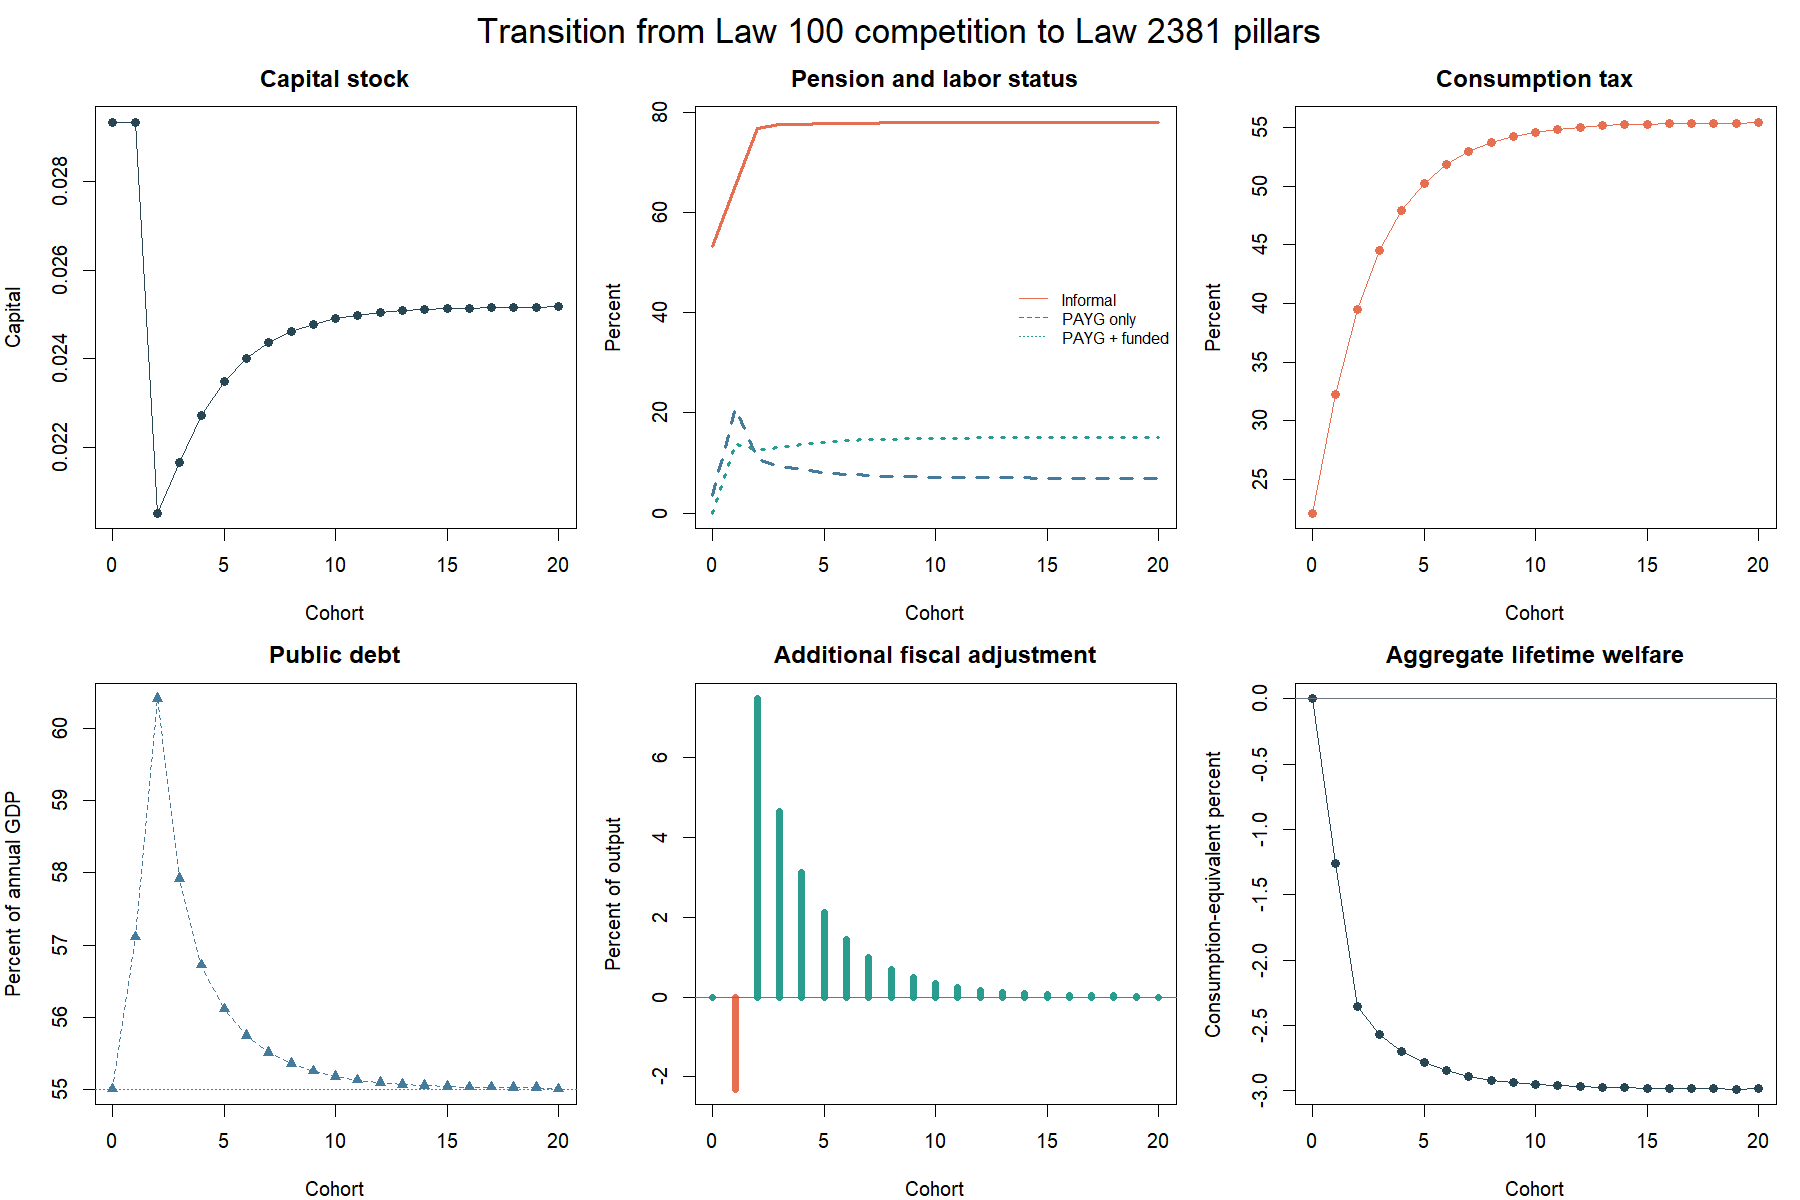
\includegraphics[width=\textwidth]{figures/policy_transition_trajectories.png}
\caption{Transition from Law 100 to the pillar system}\label{fig:transition}
\begin{minipage}{0.94\textwidth}\footnotesize
Notes: One cohort is one model period of approximately 40 years. Public debt is measured as a
share of annual GDP; the horizontal reference is the 55 percent legal anchor. The additional
fiscal adjustment is $100A_t/Y_t$ and is zero in both endpoints.
\end{minipage}
\end{figure}

The path no longer has the alternating ``accordion'' pattern. The fiscal wedge rises from
22.1 percent to 32.3 percent for cohort 1, 39.5 percent for cohort 2, and 55.4 percent in the
limit. Informality rises in the same damped direction. Capital falls sharply when the first
new pension balances mature, reaches 0.0205 for cohort 2, and converges from below to 0.0252.
Debt initially overshoots, peaking at 60.4 percent of annual GDP for cohort 2, and then returns
to 55 percent.

\begin{table}[htbp]\centering
\caption{Selected points: transition to pillars}\label{tab:transition}
\footnotesize\setlength{\tabcolsep}{3pt}
\begin{tabular}{lrrrrr}
\toprule Outcome&Law 100&Cohort 1&Cohort 2&Cohort 5&Steady state\\ \midrule
Informal share&0.5318&0.6538&0.7685&0.7772&0.7795\\
PAYG-only share&0.0344&0.2082&0.1074&0.0811&0.0697\\
Mixed share&0.0000&0.1380&0.1240&0.1417&0.1508\\
Fiscal wedge&0.2214&0.3227&0.3951&0.5024&0.5544\\
Capital stock&0.02932&0.02932&0.02054&0.02349&0.02518\\
Debt / annual GDP&0.5500&0.5711&0.6041&0.5611&0.5500\\
Additional adjustment / output (percent)&0.00&$-2.31$&7.47&2.12&0.00\\
Aggregate welfare CEV (percent)&0.00&$-1.26$&$-2.36$&$-2.79$&$-2.99$\\
\bottomrule
\end{tabular}
\end{table}

The additional fiscal instrument changes sign once: cohort 1 uses temporary fiscal space of
2.3 percent of output, whereas cohort 2 requires an adjustment of 7.5 percent as inherited
obligations come due. The adjustment then decays to zero. The terminal gap is
$4.00\times10^{-4}$, the debt-identity residual is zero to machine precision, and the maximum
fiscal-rule residual is $4.91\times10^{-5}$. Capital, debt, the wedge, and informality have at
most one direction reversal; a two-cycle is not an admissible solution.

\subsection{Transition to a fully funded formal system}

Figure~\ref{fig:fundedtransition} repeats the experiment with the full 16 percent contribution
credited to individual accounts. New cohorts earn no PAYG rights, but the government honors
Law 100 benefits already accrued and retains the solidarity benefit.

\begin{figure}[htbp]\centering
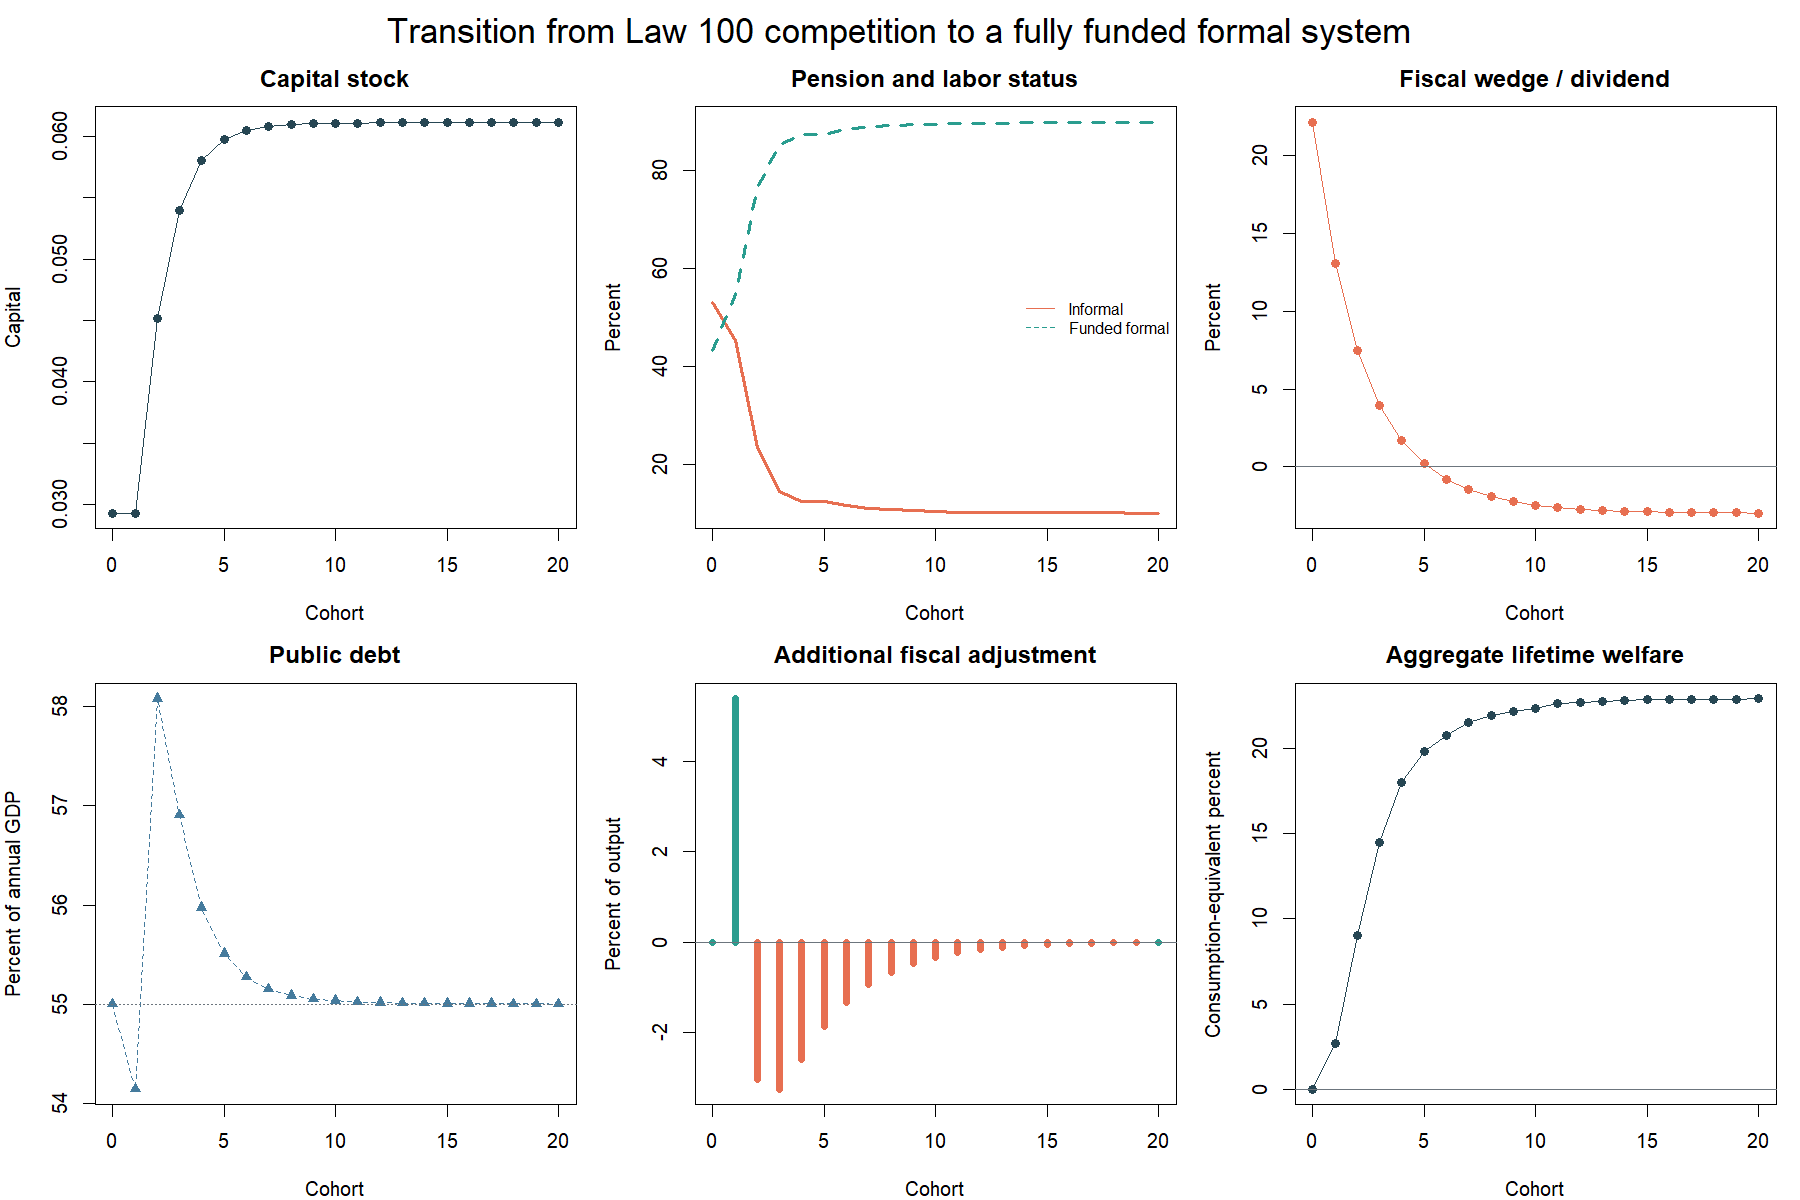
\includegraphics[width=\textwidth]{figures/policy_funded_transition_trajectories.png}
\caption{Transition from Law 100 to a fully funded formal system}\label{fig:fundedtransition}
\begin{minipage}{0.94\textwidth}\footnotesize
Notes: A negative fiscal wedge is reported as a model-implied dividend. It does not overturn
consumption taxes or other statutory taxes outside the model.
\end{minipage}
\end{figure}

The contrast is immediate. Informality falls to 45.3 percent for cohort 1, 23.5 percent for
cohort 2, and 10.2 percent in the steady state. Capital rises monotonically after the
predetermined first cohort, reaching 0.0452 for cohort 2 and 0.0611 in the limit. The fiscal
wedge falls through zero between cohorts 5 and 10. Debt peaks at 58.1 percent of annual GDP
and returns to the same 55 percent anchor. Aggregate welfare rises 2.7 percent for cohort 1,
9.0 percent for cohort 2, and 22.9 percent in the stationary allocation. The terminal and
maximum fiscal-rule gaps are $2.04\times10^{-4}$ and $4.00\times10^{-6}$.

\begin{figure}[htbp]\centering
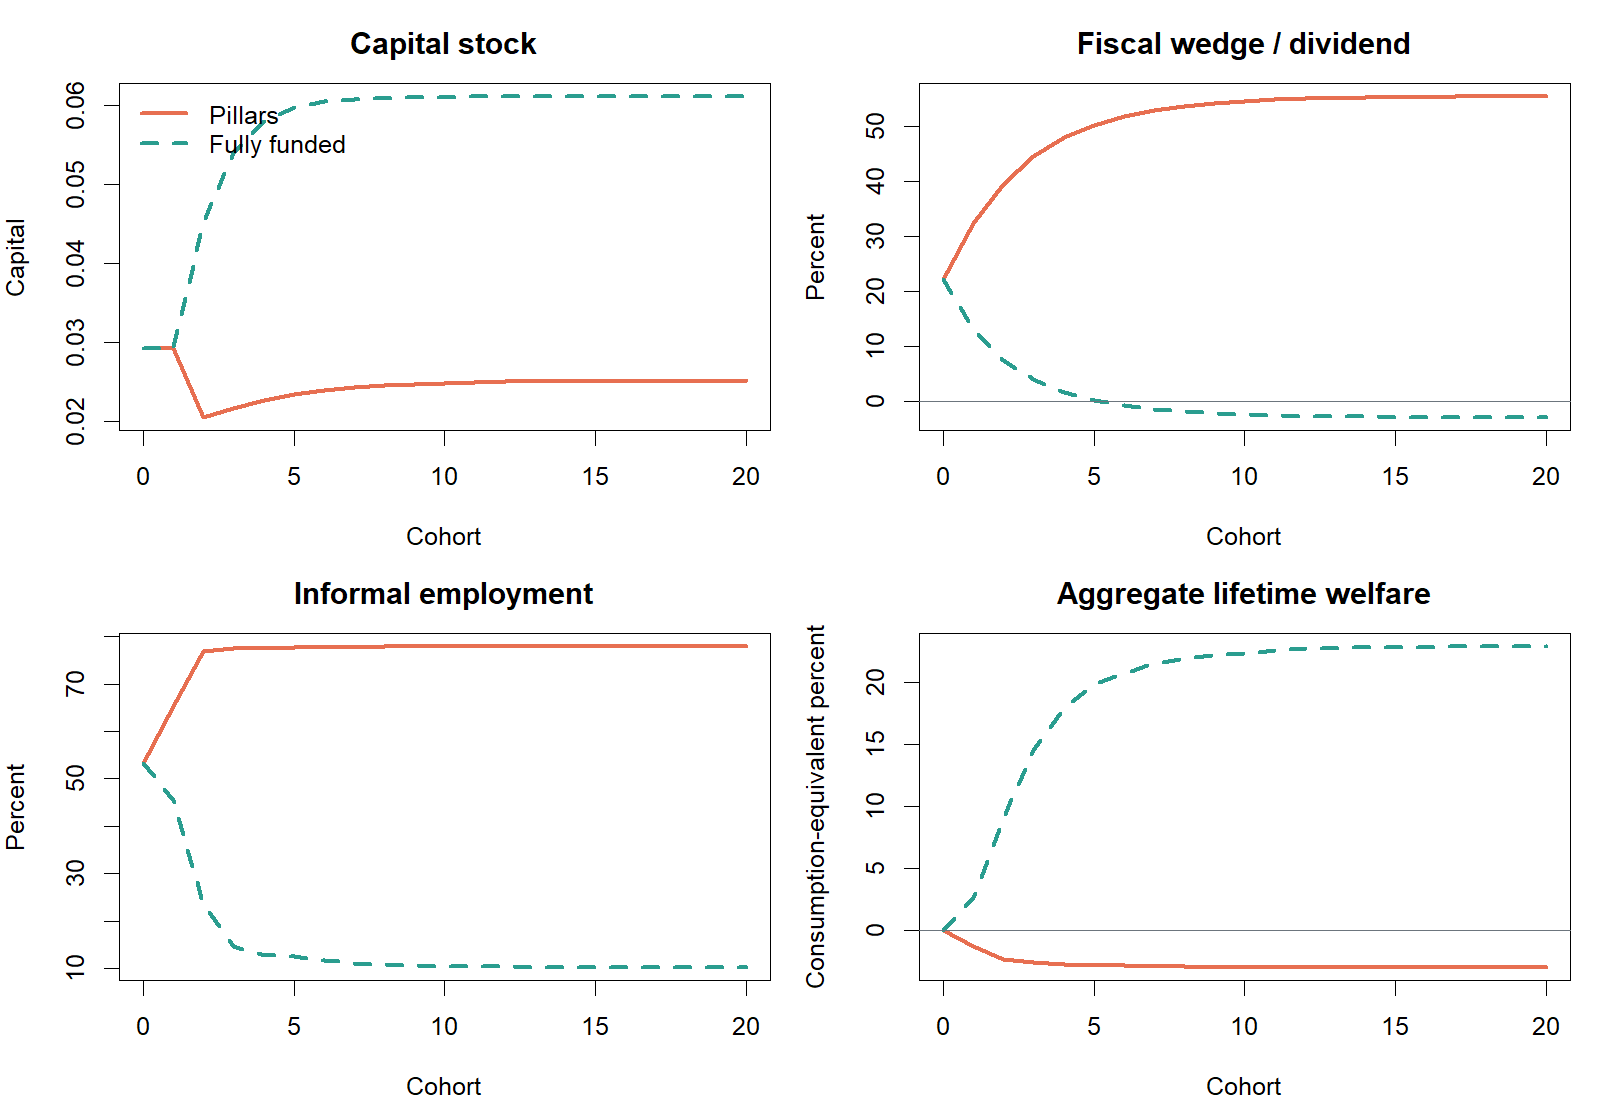
\includegraphics[width=0.94\textwidth]{figures/policy_reform_comparison.png}
\caption{Pillars and full funding: transition comparison}\label{fig:reformcomparison}
\end{figure}

\subsection{Wage and welfare distributions}

Figures~\ref{fig:wages}--\ref{fig:stationarydistribution} show that aggregate paths conceal
large within-cohort differences. Under pillars, the first reform cohort loses 1.26 percent in
aggregate, but its tenth percentile loses 12.1 percent and its ninetieth percentile gains 2.4
percent. At the pillar endpoint, aggregate welfare is 2.99 percent below Law 100; 12.2 percent
of types gain, the tenth percentile loses 20.5 percent, and the ninetieth percentile gains 1.5
percent. Those already old at the pillar reform lose 3.6 percent in aggregate even though the
upper tail benefits from the solidarity transfer.

\begin{figure}[htbp]\centering
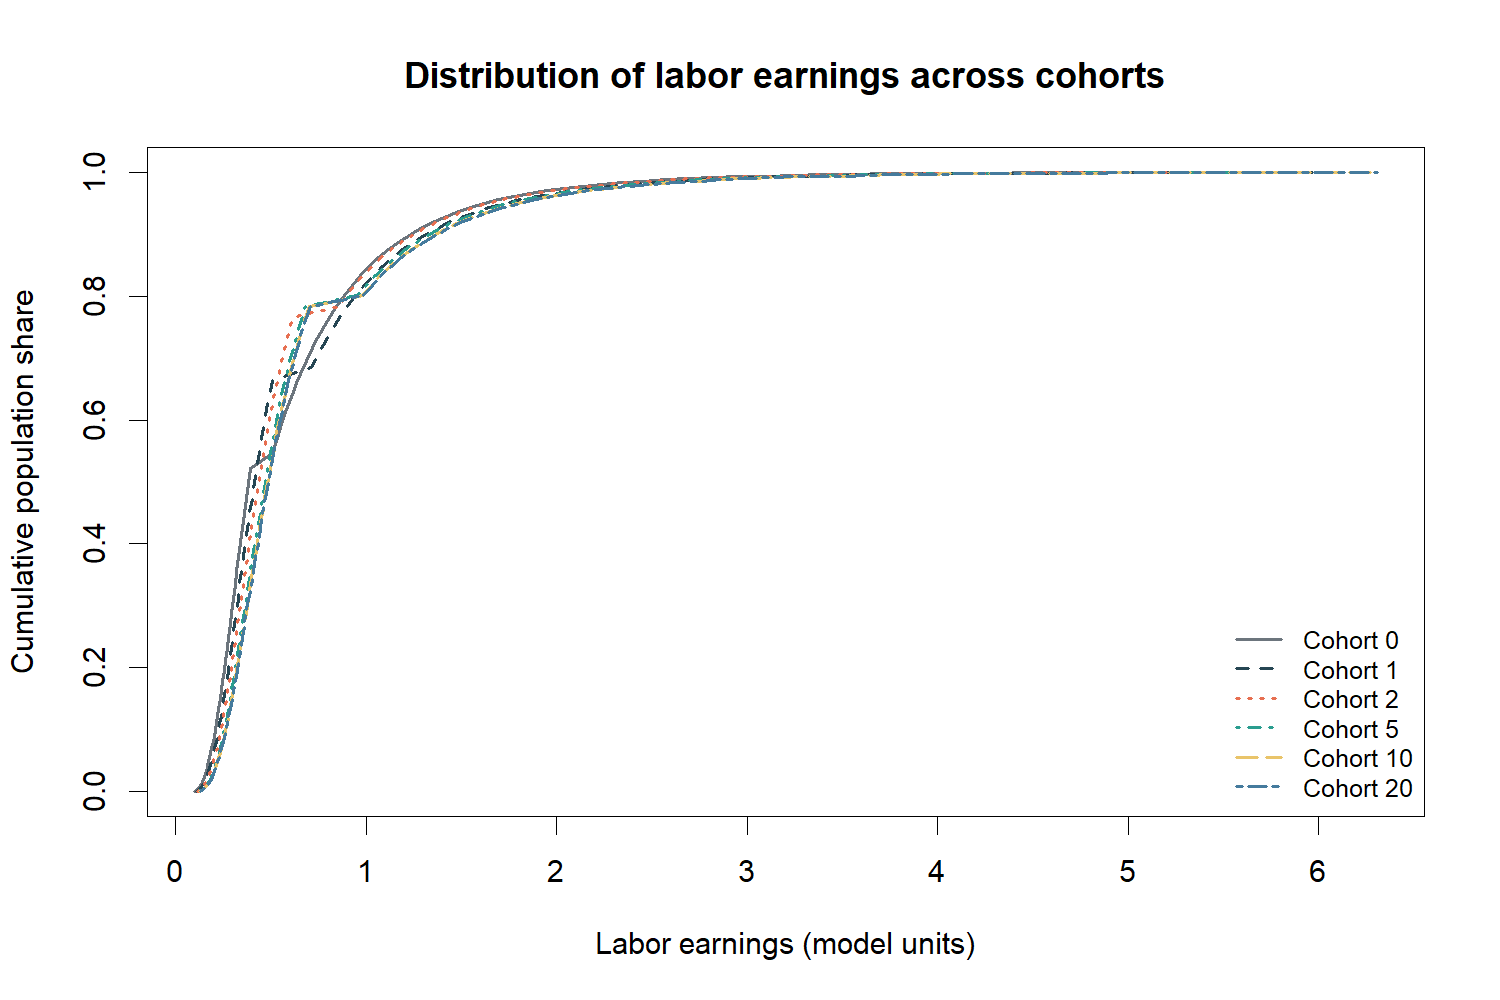
\includegraphics[width=0.88\textwidth]{figures/policy_wage_distribution.png}
\caption{Distribution of labor earnings during the pillar transition}\label{fig:wages}
\end{figure}

\begin{figure}[htbp]\centering
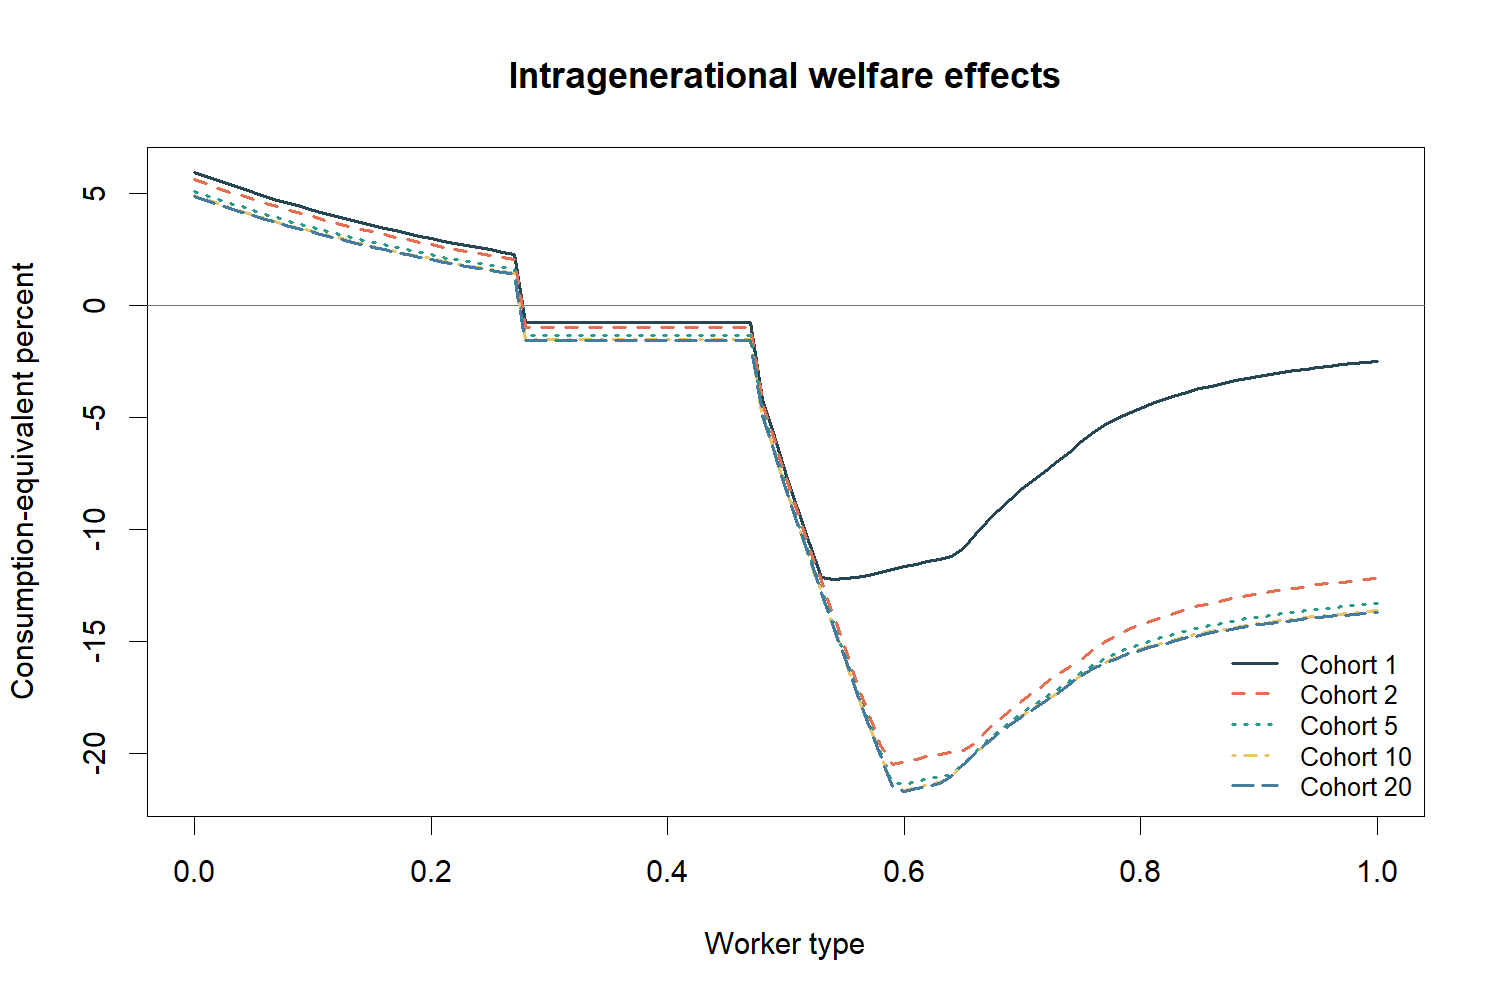
\includegraphics[width=0.88\textwidth]{figures/policy_welfare_distribution.png}
\caption{Intragenerational welfare during the pillar transition}\label{fig:intragenerational}
\end{figure}

\begin{figure}[htbp]\centering
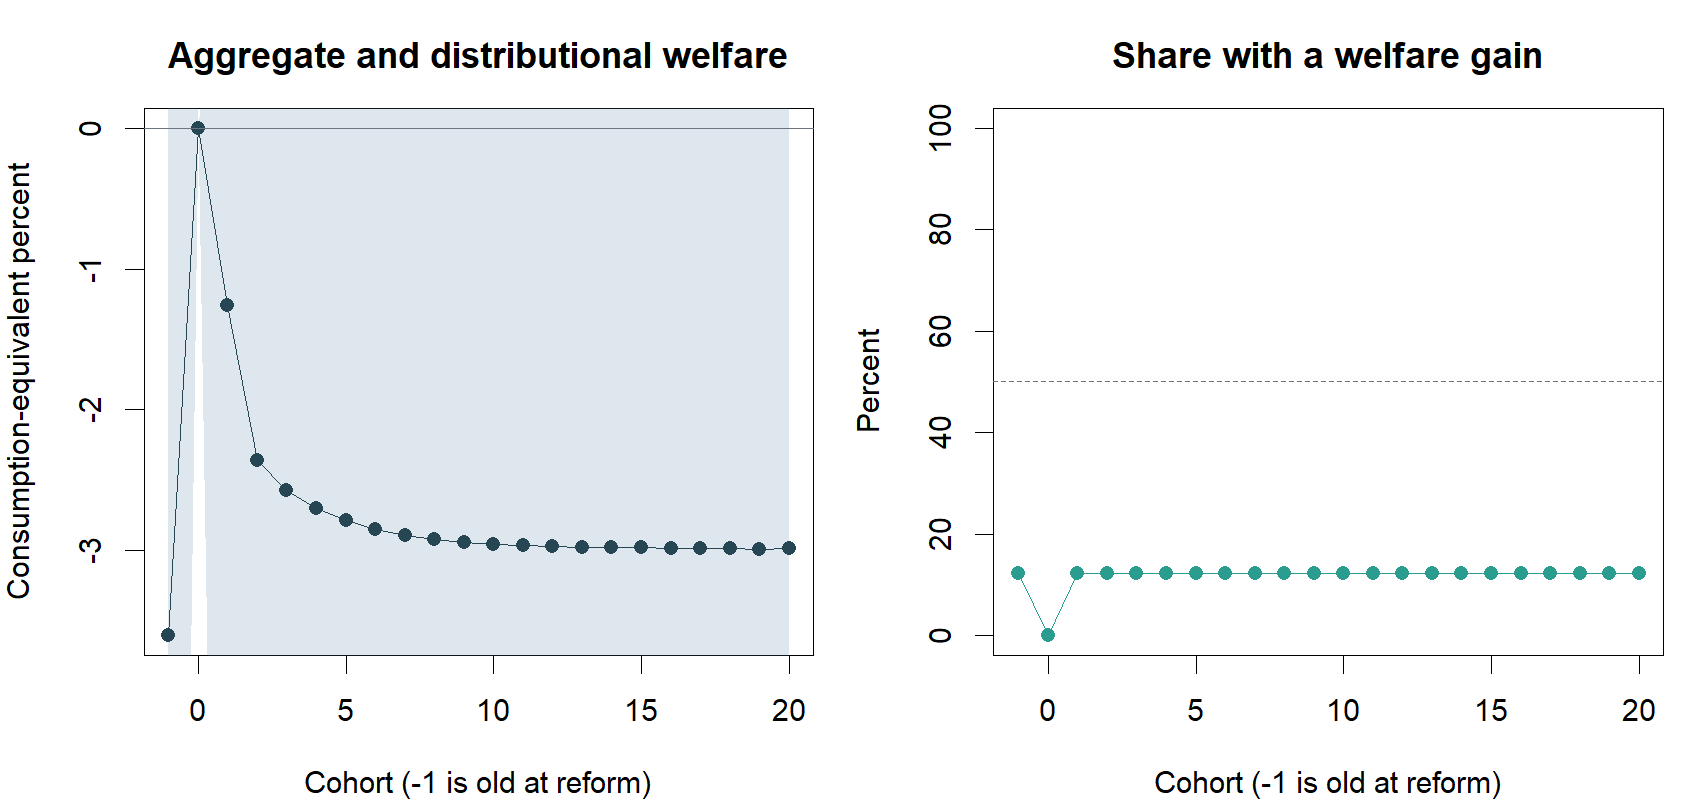
\includegraphics[width=\textwidth]{figures/policy_intergenerational_welfare.png}
\caption{Pillar transition: intergenerational welfare and share of winners}\label{fig:intergenerational}
\begin{minipage}{0.94\textwidth}\footnotesize
Notes: Welfare uses experienced utility. The shaded area spans the tenth to ninetieth
percentile of individual consumption-equivalent changes.
\end{minipage}
\end{figure}

The fully funded counterfactual is also heterogeneous early in the transition. Cohort 1 gains
2.7 percent in aggregate, but 32.8 percent of types lose slightly. By cohort 5 every type
gains. At the endpoint, the aggregate gain is 22.9 percent, the tenth percentile gains 7.9
percent, and the median gains 52.6 percent. Figure~\ref{fig:stationarydistribution} compares
stationary earnings distributions and type-level welfare profiles directly. The result is not
a Pareto theorem: it is conditional on the model's contribution valuation, fiscal incidence,
and omitted transition costs.

\begin{figure}[htbp]\centering
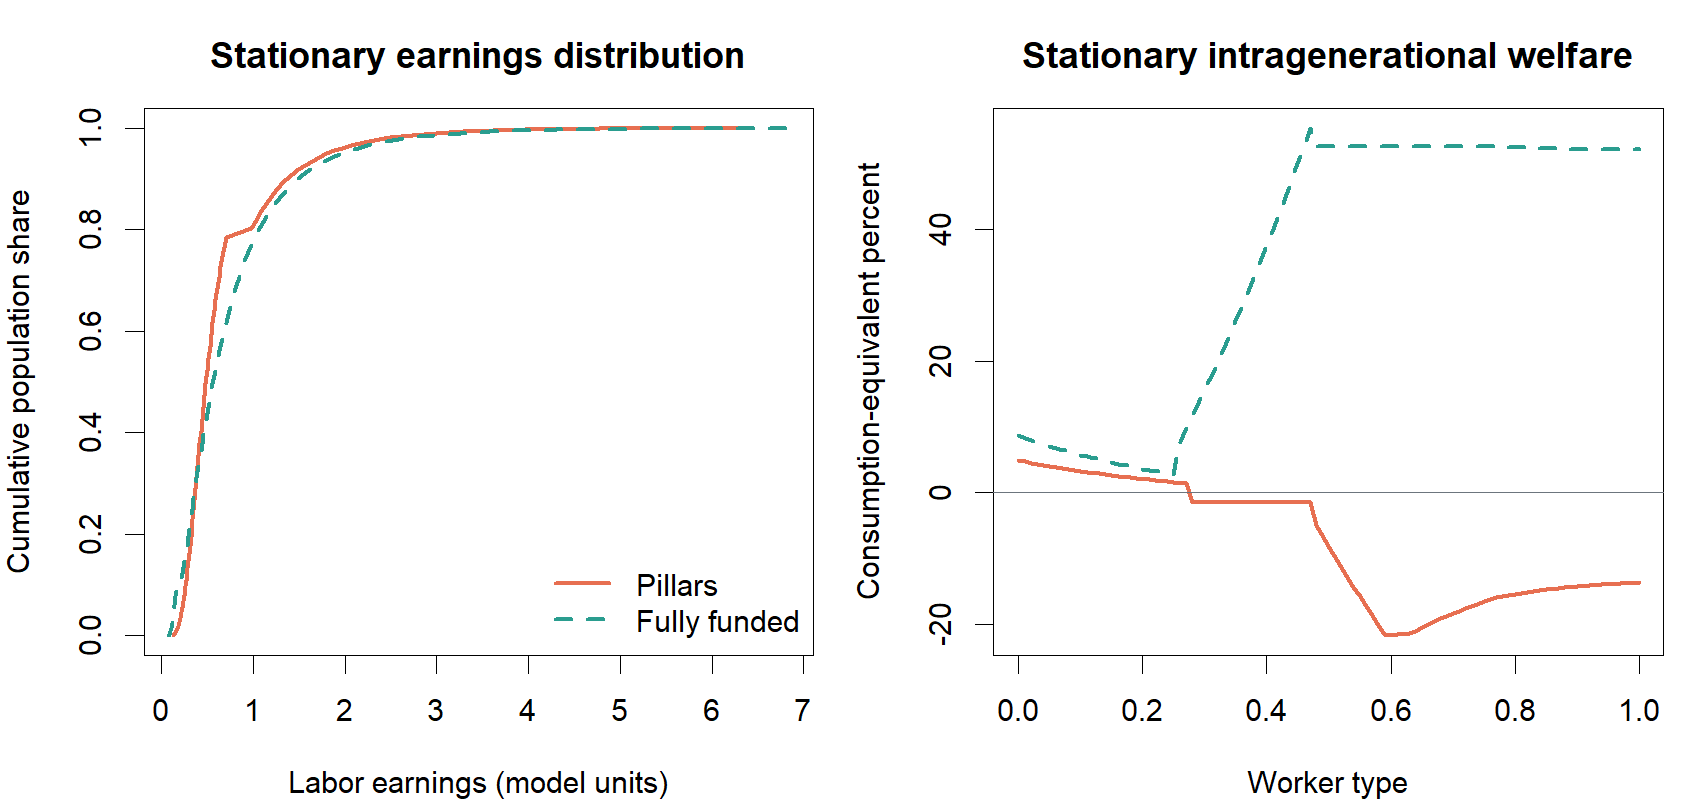
\includegraphics[width=0.94\textwidth]{figures/policy_stationary_distribution_comparison.png}
\caption{Stationary earnings and intragenerational welfare}\label{fig:stationarydistribution}
\end{figure}
\section{Conclusion}

Moving from competing regimes to pillars changes more than pension assignment. Under Law
100, informality, capitalization, and PAYG coexist because portability and eligibility create
comparative advantage across worker types. Under Law 2381, PAYG becomes mandatory up to 2.3
minimum wages and only higher earnings generate funded balances. In the model, that design
reduces funded saving substantially, raises informality, and contracts both output and the
fiscal base.

The decomposition matters. The pillar steady state does not eliminate voluntary saving and it
does not enlarge the net PAYG cash deficit. Voluntary saving almost triples and the PAYG
deficit falls. Nevertheless, funded capital falls 70 percent, total capital falls 14 percent,
and the consumption-tax base falls 44 percent as informality rises. The 55 percent stationary
tax is therefore an equilibrium feedback among the composition of saving, formality, and the
fiscal base. Treating it as the direct accounting cost of PAYG would be incorrect.

The two-instrument fiscal closure removes the former numerical accordion. The consumption
wedge follows a smooth bounded path, while a temporary primary-balance instrument stabilizes
public debt at the legal 55 percent anchor. Debt, taxes, labor status, and capital converge in
both reforms, and the additional adjustment vanishes at each endpoint. This is a disciplined
transition closure, but it does not identify which expenditure cuts or non-distortionary
revenues would implement $A_t$ in practice.

The fully funded counterfactual reverses the central pillar mechanisms: capital more than
doubles, informality falls to 10 percent, and stationary welfare rises 23 percent. Those large
gains are informative about the model's mechanism, not a policy ranking that can be exported
unchanged. The experiment omits administrative fees, annuity-market risk, portfolio choice,
minimum-return guarantees, and a detailed financing plan for legacy obligations. Its residual
fiscal dividend should be read as unused fiscal space inside the model.

Five cautions remain. First, Law 2381 has not entered into force, so the pillar exercise is
counterfactual. Second, one period is about 40 years; the paths are generational, not annual
forecasts. Third, 55 percent is the statutory long-run debt anchor, not current debt, and the
2026--2027 escape clause remains active. Fourth, setting $\omega_B=0$ prevents mechanical
domestic crowding out and is an identifying assumption. Fifth, the benefit multiplier,
minimum-wage normalization, contribution histories, and the transition adjustment are not
identified by the available calibration source.

The next step is a five-year multi-cohort model with age, sex, contribution histories,
semicontributory rules, debt maturity, and an explicit menu of fiscal instruments. That
extension would show whether the qualitative comparison survives with annual legal flows,
legacy PAYG liabilities, and empirically calibrated domestic absorption. The present model's
main contribution is narrower: it separates pension design from an unstable fiscal closure
and makes the saving, informality, tax-base, and welfare mechanisms auditable.

\appendix
\section{Numerical algorithm}

\subsection{Household alternatives}

For each candidate aggregate state $(K,N_f,N_s,\tau_c)$, the algorithm computes prices and
solves household problems at every diagnostic type. Under Law 100 the alternatives are
informality, formal funded employment, and formal PAYG employment. Under pillars, the two
choices are informality and the statutory PAYG--funded package. Under the fully funded
counterfactual, the formal package sends the full contribution to the individual account.
Each problem imposes nonnegative voluntary saving and positive consumption. Choice maximizes
decision utility, while welfare uses experienced utility.

\subsection{Locating endogenous thresholds}

The diagnostic grid identifies every interval in which the selected alternative or pension
classification changes. A scalar root finder solves the relevant utility equality within each
bracket. Roots and the statutory pillar-income threshold are added to the quadrature nodes.
Choice is evaluated at interval midpoints and held fixed only inside those root-bounded
intervals. The method neither assumes the number of crossings nor imposes their order.

\subsection{Stationary general equilibrium}

Given the exact intervals, trapezoidal quadrature aggregates labor, consumption, voluntary
saving, funded contributions, PAYG flows, and welfare. The update map is
\begin{equation}
(K,N_f,N_s,\tau_c)
\longmapsto
(\widehat K,\widehat N_f,\widehat N_s,\widehat\tau_c).
\end{equation}
At each candidate allocation, output maps the annual legal targets into
$\bar B=0.55Y/H$ and $\overline{PB}=0.002Y$. Gross household assets are converted to productive
capital using \eqref{eq:crowding}, and the stationary fiscal wedge solves the consolidated
budget including the primary-surplus target. Damped updates continue until the four state
variables and fixed-point residuals satisfy tolerance.

The publication script solves 101 types and uses that allocation to initialize 201 types.
Validation requires positive consumption, nonnegative saving, normalized regime shares,
regime-appropriate threshold structure, the income identity, the debt anchor, the primary
balance target, and maximum fixed-point residual below $5\times10^{-5}$. The four reported
states---Law 100, central pillars, pillar stress, and full funding---all pass.

\subsection{Transition path iteration}

Let $T=20$. The initial capital stock and public debt are predetermined by the Law 100 steady
state, including $HB_0/Y_0=0.55$. From cohort 1 onward, entrants face either pillar or fully
funded parameters. Those old at announcement retain their Law 100 contributory rights and
accumulated saving.

For a candidate sequence
\[
\{K_t,N_{ft},N_{st},\tau_{ct}\}_{t=0}^{T},
\]
the algorithm performs a backward-looking household/forward fiscal sweep:
\begin{enumerate}
\item compute current prices and the candidate next-period return;
\item solve each cohort's household problem and integrate gross assets and labor;
\item update the fiscal wedge through \eqref{eq:fiscalrule};
\item compute $PB_t^{raw}$, $PB_t^*$, and $A_t$ using
\eqref{eq:pbrule}--\eqref{eq:fiscaladjustment};
\item advance debt using \eqref{eq:debt} and map gross assets into capital using
\eqref{eq:crowding}.
\end{enumerate}
Debt is generated by the forward sweep rather than guessed independently. A positive $A_t$
is an additional primary adjustment; the endpoint restriction is $A_0=A_T=0$.

Real paths are updated with an old-iterate weight of 0.75 and fiscal paths with a weight of
0.50. These are numerical relaxation parameters and do not alter the fixed point. A saved
validated path may be used as a warm start, but every equation is reevaluated. Iteration stops
only when the maximum state change is below $10^{-4}$ and the fiscal-rule residual below
$2\times10^{-4}$.

The joint terminal gap uses an absolute fiscal-wedge error because the fully funded target is
close to zero:
\begin{equation}
\Delta_T=\max\left\{
\frac{|\widehat K_T-\bar K|}{\bar K},
\frac{|\widehat B_T-\bar B|}{\bar K},
|\widehat\tau_{c,T-1}-\bar\tau_c|
\right\}.
\label{eq:terminaltest}
\end{equation}
A path is accepted only if the internal fixed point converges, $\Delta_T<10^{-3}$, and the
maximum debt-identity and fiscal-rule residuals are below $2\times10^{-4}$. As an additional
anti-accordion check, capital, debt, the wedge, and informality may have no more than two
direction reversals. The pillar path has one; the fully funded path has none. Their terminal
gaps are $4.00\times10^{-4}$ and $2.04\times10^{-4}$, respectively. Debt-identity residuals
are zero to machine precision, and maximum fiscal-rule residuals are
$4.91\times10^{-5}$ and $4.00\times10^{-6}$.

\subsection{Distributional accounting}

The code retains 101 type-level observations for every transition cohort. Population weights
are quadrature weights from $f(i)$. Reports include weighted wage quantiles, Gini coefficients,
winner shares, and welfare percentiles. Normative welfare uses experienced utility $W$, not
the present-biased decision utility $V$. For $\sigma\neq1$, the consumption-equivalent change
under reform $r$ relative to Law 100 is
\begin{equation}
\lambda_r(i)=
\left[\frac{W^r(i)}{W^{100}(i)}\right]^{1/(1-\sigma)}-1.
\end{equation}
Those old at reform receive an old-age-only equivalent; young cohorts receive a lifetime
equivalent. Aggregate equivalents are computed from weighted aggregate utilities and are not
the arithmetic mean of individual equivalents.
\bibliographystyle{chicago}
\bibliography{references}
\end{document}
